%%%%%%%%%%%%%%%%%%%%%%%%%%%%%%%%%%%
%This is the LaTeX ARTICLE template for RSC journals
%Copyright The Royal Society of Chemistry 2016
%%%%%%%%%%%%%%%%%%%%%%%%%%%%%%%%%%%

\documentclass[twoside,twocolumn,9pt]{article}
\usepackage{extsizes}
\usepackage[super,sort&compress,comma]{natbib} 
\usepackage[version=3]{mhchem}
\usepackage[left=1.5cm, right=1.5cm, top=1.785cm, bottom=2.0cm]{geometry}
\usepackage{balance}
\usepackage{times,mathptmx}
\usepackage{sectsty}
\usepackage{graphicx} 
\usepackage{lastpage}
\usepackage[format=plain,justification=justified,singlelinecheck=false,font={stretch=1.125,small,sf},labelfont=bf,labelsep=space]{caption}
\usepackage{float}
\usepackage{fancyhdr}
\usepackage{fnpos}
\usepackage[english]{babel}
\usepackage{array}
\usepackage{droidsans}
\usepackage{charter}
\usepackage[T1]{fontenc}
\usepackage[usenames,dvipsnames]{xcolor}
\usepackage{setspace}
\usepackage[compact]{titlesec} % added captionof package to add captions to equations
%%%Please don't disable any packages in the preamble, as this may cause the template to display incorrectly.%%%


\usepackage{epstopdf}%This line makes .eps figures into .pdf - please comment out if not required.

\definecolor{cream}{RGB}{222,217,201}

%%%%%%%%%%%%%%%%%%% MACRO DEFINITIONS%%%%%%%%%%%%%%%%%%%%%%%%%%%%%%%%%%%%%%%%%%

%============================== Document macro =======================================
\newcommand{\doc}[1]{%
	\begin{document}
		#1
	\end{document}}
%=====================================================================================                    

%======================= NICER ITEMIZE/ENUMERATE SYNTAX ==============================
\newcommand{\ol}[1]{\begin{enumerate}#1\end{enumerate}}
\newcommand{\ul}[1]{\begin{itemize}#1\end{itemize}}
\newcommand{\li}[1]{\item {#1}}
\newlength{\shiftwidth}
\setlength{\shiftwidth}{3em}
\newcommand{\info}[1]{\par\hspace*{#1\shiftwidth}$\bullet$\quad}
%=====================================================================================

%========================== NICER IMAGE INCLUDE SYNTAX================================
\newcommand{\fig}[2]{%
	\begin{figure}
		\centering\includegraphics[#1]{#2}
		\label{fig:#2}
	\end{figure}}
	\newcommand{\figc}[3]{%
		\begin{figure}
			\centering\includegraphics[#1]{#2}
			\caption{\footnotesize #3}
			\label{fig:#2}
		\end{figure}}
%=====================================================================================
		
%============================= LAZY MULTIICOL ENVIRONMENT ============================
\newcommand{\mcol}[2]{%
	\begin{multicols}{#1}
		#2
	\end{multicols}
		}
%=====================================================================================
		
%============================== Shorter vspace ======================================
\newcommand{\vs}[1]{%
	\vspace{#1}
}
\newcommand{\vst}[1]{%
	\vspace*{#1}
}
%===================================================================================
		
%============================== Lazy frame =========================================
\newcommand{\f}[1]{%
	\begin{frame}
		#1
	\end{frame}
}
\newcommand{\ft}[2]{%
	\begin{frame}{#1}
		#2
	\end{frame}
}
%=================================================================================== 

%========================== Simple table ===========================================
\newcommand{\tab}[2]{%
	\begin{table}[!htbp]
		\begin{tabular}{#1}\hline
			#2
		\end{tabular}
	\end{table}}
%===============================================================================	
	
%=========================== BOLD ====================================
\newcommand{\bold}[1]{\textbf{#1}}
%========================================================================
\begin{document}

\pagestyle{fancy}
\thispagestyle{plain}
\fancypagestyle{plain}{

%%%HEADER%%%
\fancyhead[C]{
\includegraphics[width=18.5cm]{head_foot/header_bar}}
\fancyhead[L]{\hspace{0cm}\vspace{1.5cm}
\includegraphics[height=30pt]{head_foot/journal_name}}
\fancyhead[R]{\hspace{0cm}\vspace{1.7cm}
\includegraphics[height=55pt]{head_foot/RSC_LOGO_CMYK}}
\renewcommand{\headrulewidth}{0pt}
}
%%%END OF HEADER%%%

%%%PAGE SETUP - Please do not change any commands within this section%%%
\makeFNbottom
\makeatletter
\renewcommand\LARGE{\@setfontsize\LARGE{15pt}{17}}
\renewcommand\Large{\@setfontsize\Large{12pt}{14}}
\renewcommand\large{\@setfontsize\large{10pt}{12}}
\renewcommand\footnotesize{\@setfontsize\footnotesize{7pt}{10}}
\makeatother

\renewcommand{\thefootnote}{\fnsymbol{footnote}}
\renewcommand\footnoterule{\vspace*{1pt}% 
\color{cream}\hrule width 3.5in height 0.4pt \color{black}\vspace*{5pt}} 
\setcounter{secnumdepth}{5}

\makeatletter 
\renewcommand\@biblabel[1]{#1}            
\renewcommand\@makefntext[1]% 
{\noindent\makebox[0pt][r]{\@thefnmark\,}#1}
\makeatother 
\renewcommand{\figurename}{\small{Fig.}~}
\sectionfont{\sffamily\Large}
\subsectionfont{\normalsize}
\subsubsectionfont{\bf}
\setstretch{1.125} %In particular, please do not alter this line.
\setlength{\skip\footins}{0.8cm}
\setlength{\footnotesep}{0.25cm}
\setlength{\jot}{10pt}
\titlespacing*{\section}{0pt}{4pt}{4pt}
\titlespacing*{\subsection}{0pt}{15pt}{1pt}
%%%END OF PAGE SETUP%%%

%%%FOOTER%%%
\fancyfoot{}
\fancyfoot[LO,RE]{\vspace{-7.1pt}
\includegraphics[height=9pt]{head_foot/LF}}
\fancyfoot[CO]{\vspace{-7.1pt}\hspace{13.2cm}
\includegraphics{head_foot/RF}}
\fancyfoot[CE]{\vspace{-7.2pt}\hspace{-14.2cm}
\includegraphics{head_foot/RF}}
\fancyfoot[RO]{\footnotesize{\sffamily{1--\pageref{LastPage} ~\textbar  \hspace{2pt}\thepage}}}
\fancyfoot[LE]{\footnotesize{\sffamily{\thepage~\textbar\hspace{3.45cm} 1--\pageref{LastPage}}}}
\fancyhead{}
\renewcommand{\headrulewidth}{0pt} 
\renewcommand{\footrulewidth}{0pt}
\setlength{\arrayrulewidth}{1pt}
\setlength{\columnsep}{6.5mm}
\setlength\bibsep{1pt}
%%%END OF FOOTER%%%

%%%FIGURE SETUP - please do not change any commands within this section%%%
\makeatletter 
\newlength{\figrulesep} 
\setlength{\figrulesep}{0.5\textfloatsep} 

\newcommand{\topfigrule}{\vspace*{-1pt}% 
\noindent{\color{cream}\rule[-\figrulesep]{\columnwidth}{1.5pt}} }

\newcommand{\botfigrule}{\vspace*{-2pt}% 
\noindent{\color{cream}\rule[\figrulesep]{\columnwidth}{1.5pt}} }

\newcommand{\dblfigrule}{\vspace*{-1pt}% 
\noindent{\color{cream}\rule[-\figrulesep]{\textwidth}{1.5pt}} }

\makeatother
%%%END OF FIGURE SETUP%%%

%%%TITLE, AUTHORS AND ABSTRACT%%%
\twocolumn[
  \begin{@twocolumnfalse}
\vs{3cm}
\sffamily
\begin{tabular}{m{4.5cm} p{13.5cm} }


\includegraphics{head_foot/DOI} & \noindent\LARGE{\bold{A Method for Studying the Diffusion of Quaternary Ammonium Cations Through Polyelectrolyte Phases$^\dag$}} \\%Article title goes here instead of the text "This is the title"
\vs{0.3cm} & \vs{0.3cm} \\

 & \noindent\large{Alexander M. Papiez,$^{\ast}$\textit{$^{a}$} Justin J. B. Perry,\textit{$^{b\ddag}$} and Les R. Dix\textit{$^{a}$}} \\%Author names go here instead of "Full name", etc.


\includegraphics{head_foot/dates} & \noindent\normalsize{The mobility of organic cations in polymeric phases is an important property to consider when using these materials as active ingredients in coatings. Here we describe a method for extracting such compounds from polymeric samples and how analysis of these extracts can yield insights about the diffusivity of molecules in a polymeric phase.} \\%The abstrast goes here instead of the text "The abstract should be..."

\end{tabular}

 \end{@twocolumnfalse} \vspace{0.6cm}

  ]
%%%END OF TITLE, AUTHORS AND ABSTRACT%%%

%%%FONT SETUP - please do not change any commands within this section
\renewcommand*\rmdefault{bch}\normalfont\upshape
\rmfamily
\section*{}
\vspace{-1cm}


%%%FOOTNOTES%%%

\footnotetext{\textit{$^{a}$~Address, Address, Town, Country. Fax: XX XXXX XXXX; Tel: XX XXXX XXXX; E-mail: xxxx@aaa.bbb.ccc}}
\footnotetext{\textit{$^{b}$~Address, Address, Town, Country. }}

%Please use \dag to cite the ESI in the main text of the article.
%If you article does not have ESI please remove the the \dag symbol from the title and the footnotetext below.
\footnotetext{\dag~Electronic Supplementary Information (ESI) available: [details of any supplementary information available should be included here]. See DOI: 10.1039/b000000x/}
%additional addresses can be cited as above using the lower-case letters, c, d, e... If all authors are from the same address, no letter is required

\footnotetext{\ddag~Additional footnotes to the title and authors can be included \textit{e.g.}\ `Present address:' or `These authors contributed equally to this work' as above using the symbols: \ddag, \textsection, and \P. Please place the appropriate symbol next to the author's name and include a \texttt{\textbackslash footnotetext} entry in the the correct place in the list.}


%%%END OF FOOTNOTES%%%

%%%MAIN TEXT%%%%
%\subsection{This is the subsection heading style}
%Section headings can be typeset with and without numbers.\cite{Abernethy2003}

%\subsubsection{This is the subsubsection style.~~} These headings should end in a full point.  

%\paragraph{This is the next level heading.~~} For this level please use \texttt{\textbackslash paragraph}. These headings should also end in a full point.

\section{Introduction}
Diffusion in polymeric phases is an important phenomenon which influences many fields. The ability to control the release of active compounds from a polymeric vehicle may be influenced by the diffusivity of these compounds, especially when strong interactions exist between the active compound and the vehicle. Particularly interesting are those cases in which these interactions can be modified to tune the diffusivity of the mobile compound. 

In order to assess how different structural features assess the diffusivity of an analyte, the kinetics of analyte release must be measured. The methods used to effect this measurement are highly dependant on both the nature and quantity of the analyte of interest. 

\begin{table}[h]
\small
  \caption{\ Some typical methods used to detect different types of analyte}
  \label{tbl:example}
  \begin{tabular*}{0.48\textwidth}{@{\extracolsep{\fill}}lll}
    \hline
    Analyte & Detection Method & Sensitivity \\
    \hline
    Transition metal & Flame Photometry & 10-1000 ppm\\
                     & Flame AAS        & 1-100 ppm\\
                     & Flame AES        & < 1 ppm \\
    Organic Cations  & HPLC-MS          & 10ppb - 10 ppm\\
                     & GC-MS            & 10ppb - 10 ppm\\
                     & qNMR             & 10 - 1000 ppm\\
                     \hline
  \end{tabular*}
\end{table}

While HPLC-MS and GC-MS are by far the most sensitive techniques for the investigation of organic compounds, much time and effort must be spent developing and optimizing analyte extraction, pre-concentration and detection methods. Alternative methods, such as flame-photometry and quantitative NMR spectroscopy require less method development but are concomitantly less sensitive. The aim of this work was to establish whether the kinetics of the ion exchange of quaternary ammonium cations could be studied using a combination of flame photometry and qNMR.

\subsection{Ion Exchange}
\begin{figure}[h !]
	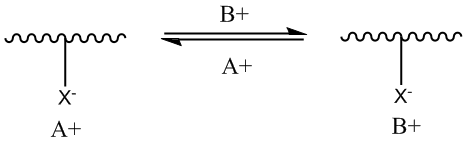
\includegraphics[width=.5\textwidth]{images/ion_exchange}
	\caption{Basic outline of the ion exchange equilibrium, where an incoming ion B+ can displace a resin associated ion A+ }
	\label{fig:ion_ex}
\end{figure}

\subsection{Basic Principle}
Ion exchange describes the phenomenon in which an ion exchange material in some initial ionic form will, in contact with a solution containing some ion of a different type to that already contained within the resin, will take-up that ion while releasing the initial ion. 

\begin{equation}
R\bar{A} + B^+ \leftrightarrow R\bar{B} + A^+
\end{equation}

This phenomenon is of great utility in a large number of industrially important processes; notably the preferential extraction of radioactive isotopes from the waste produced by nuclear reactors.

\subsection{Ion Exchange materials}
A typical ion exchange material consists of a crosslinked polymeric matrix containing acidic or basic side chains (depending upon whether cation or anion exchange is the desired behaviour of the resin). One of the most popular co-polymers used as a matrix for ion-exchange material is styrene-divinylbenzene (SDVB)(see figure \ref{fig:sdvb}).

\begin{figure}[h !]
	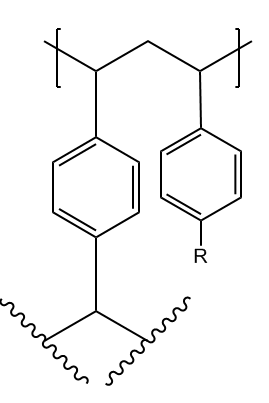
\includegraphics[height=.2\textheight]{images/sdvb}
	\centering
	\caption{The styrene-divinylbenzene co-polymer is one of the most popular skeletons for ion exchange resins. R may be any acidic or basic group, dependant upon whether cation or anion exchange functionality is desired}
	\label{fig:sdvb}
\end{figure}

SDVB based resins are particularly attractive due to the ease with which polymer beads of a well controlled size distribution may be obtained. This is achieved by inverse phase suspension free radical polymerization of the monomers in water.  As we shall later discuss, this size control is critical for the production of ion exchange resins which behave in a well defined and predictable manner.

\subsection{The Kinetics of Ion Exchange}
The kinetics of ion exchange are well understood, with the first pioneering studies undertaken by Hellferich at the beginning of the 20th century.\cite{helfferich1962} The early consensus which was established is that diffusion of ions is the rate-controlling step in ion exchange reactions. There are however two separate diffusive mechanisms which may dominate, depending on reaction conditions, the structure of the ion exchange resin and the nature of the ions undergoing exchange.

\begin{figure}[h !]
	\centering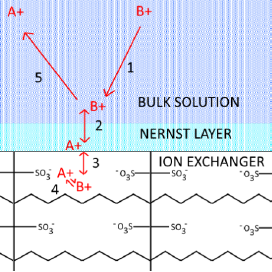
\includegraphics[height=.3\textwidth]{images/types_of_diffusion}
	\caption{Ion exchange consists of a number of steps; 1+5: diffusion of ions through the bulk solution, 2: diffusion of ions through the Nernst Layer, 3: diffusion of ions through the polymeric phase, 4: exchange of ions at the ionic polymer side chain}
	\label{fig:diftypes}
\end{figure}

Figure \ref{fig:diftypes} shows the various sub-processes which make up the overall ion exchange process. It is widely accepted that of all these processes, only diffusion through the Nernst layer and the ion exchanger itself are rate controlling (processes 2 and 3 respectively).\cite{helfferich1962} 

When studying the ion exchange reaction it is important to determine which diffusion type is rate controlling; not only are they subject to significantly different mathematical interpretations, they shed light on diffusion in different regions. In other words, to study diffusivity of a molecule within a polymeric phase, particle diffusion not film diffusion must be rate controlling. Table \ref{tab:diff_type_control} shows how the reaction conditions can be modified in order to influence which process will be rate controlling. 

\begin{table}[h !]
	\small
	\caption{The effect of different reaction conditions on the two potential rate controlling diffusion types}
	\label{tbl:example}
	\begin{tabular*}{0.48\textwidth}{@{\extracolsep{\fill}}lll}
		\hline
		Condition & Particle Diffusion & Film Diffusion\\
		          &                    & Control \\
		\hline
		Ion mobility in particle & $\propto$ mobility & No effect\\
		In bulk solution& No effect   & $\propto$ mobility \\
		Particle size& $\frac{1}{r^2}$  & $\propto \frac{1}{r}$ \\
		Capacity of exchanger  &  no effect   & $\propto \frac{1}{X}$\\
		Nature of ionic groups & $\propto$ strength of &  No effect\\
		                       &  electrostatic interaction & \\
		Degree of cross-linking & $\propto \frac{1}{crosslink degree}$  & No effect\\
		\hline
	\end{tabular*}
	\label{tab:diff_type_control}
\end{table}

\subsubsection{Fick's law}
\begin{equation}
J = -\frac{\delta\phi}{\delta x}\label{eq:2}
test
\end{equation}
\begin{equation}
\frac{\delta\phi}{\delta t} = -D\frac{\delta^2\phi}{\delta x^2}\label{eq:3}
\end{equation}

Fick, based upon Fourier's seminal treatment on the transport of heat across temperature gradients, explained the phenomenon of the diffusion of matter via Fick's first (eq \ref{eq:2}) and second (eq \ref{eq:3}) laws.

Fick's second law, describes how the concentration of a diffusing substances changes over time. In the 1940s, Boyd brought together the observations of ion exchange which had been made up to that point and derived the first
formal mathematical law describing ion exchange reaction kinetics in a distinct manner (compared to the contemporary treatment of chemical equilbria) (\ref{eq:4}).
where $F$ = Fractional exhaustion, $r$ = radius of ion exchange particle, $D_i$ = interdiffusion coefficent of the system and t = time (seconds).
\begin{equation}
F = 1 - \frac{6}{\pi^2} \sum^\infty_1 \frac{1}{n^2}e^{-D_i\pi^2n^2tr^{-2}}\label{eq:4}
\end{equation}

Boyd formulated his kinetic model of ion exchange in terms of a spherical geometry. This was beneficial for two reasons; simplification of measurement and analysis in addition to matching the geometry of ion exchange beads seen in commercial settings. For these reasons spherical geometry
often remains a standard assumption when kinetic studies are being performed.
The standard practice for elucidation of the diffusion coefficient of ions undergoing exchange was originally 
\begin{figure}[h]
	\vs{2cm}
	\centering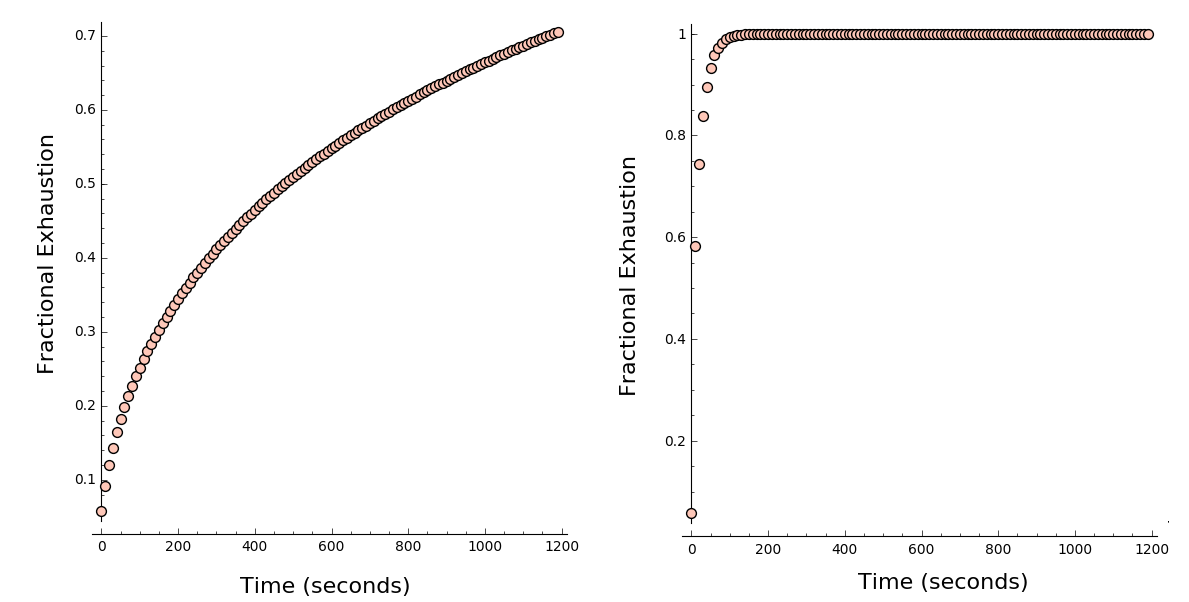
\includegraphics[width=.5\textwidth]{images/theoreticalF}
	\caption{Example of a theoretical ion exchange profile plotted from \ref{eq:4} radius of 1.25mm
		Diffusion coefficients: $1\times10^{-12}m^2s^{-1}$ (left) $7\times10^{-11}m^2s^{-1}$ (right) } 
	\label{fig:theoreticalF}
\end{figure}

The diffusion coefficient can be extracted from a F vs t curve by noting that if the diffusion coefficient is assumed to be constant (i.e. $\frac{\delta D_i}{\delta C}=0$) then equation \ref{eq:4} can be written as:

\begin{equation}
F = 1 - \frac{6}{\pi^2}\sum^{\infty}_{1}\frac{1}{n^2}e^{-n^2Bt}\label{eq:5}
\end{equation}
where $B=\frac{D_i\pi^2}{r^2}$
F can then be expressed as a function of Bt (with the form of the expression varying to accommodate changes in the significance of terms)
\begin{equation}
	F = 1 - \frac{6}{\pi^2}e^-{Bt}\ at\ high\ F\ and\ F = \frac{6}{\pi^{\frac{3}{2}}}\sqrt{Bt} - \frac{3}{\pi^2}(Bt)\ at\ low\ F\label{eq:6}
\end{equation}

We can see from \ref{eq:6} that incorrect measurements of the particle size will cause an apparent reduction in the diffusion coefficient. 

\subsubsection{Beyond Fick}
A notable omission in Boyd's work is an explicit consideration of the coulombic forces arising in the system due to the movement of charged particles. While this apparently does not diminish the power of Boyds formulae to explain ion exchange data, it is not consistent with other known behaviours of ion exchange resins. Specifically, the initial reaction velocity for an ion exchange reaction is in many cases dependent on the form the resin is in at the start of the reaction. Boyd's model cannot help us in explaining this phenomenon. 

This disparity in reaction rate can be explained by reference to the coulombic interaction of the exchanging ions and the fact that overall the system remains neutral, precluding any net charge flow. The logical conclusion from these statements is the velocity of ion ingress must exactly match that of ion egress at all times during the reaction. We know from standard chromatographic theory that a species travelling through an adsorbent phase to which it is strongly attracted will take longer to traverse that phase than if weak interactions prevailed. The same phenomenon is at work during an ion exchange reaction, and in the absence of a concentration gradient would be important in determining the drift velocity of an ion.

When two ions of like charge and significantly different mobilities are undergoing ion exchange, the velocity of one ion will influence the velocity of the other. A rapidly diffusing ion will be retarded by a slow moving one and vice versa; hence the velocity of exchange is dependant on the interaction between the ions. An oft used analogy for the phenomenon of differential ionic mobility is that of politicians moving through a crowd: the more popular (i.e. strongly interacting) individuals will tend to move slowly through the crowd while an unpopular individual might prefer to make haste. If we extend this analogy to a meeting hall in which only a certain number of politicians are permitted to reside at any one time, we find that slow moving individuals are encouraged to speed up to accommodate the wishes of their less popular colleagues while the fast-movers are prevented from leaving the hall at a sprint to keep the numbers balanced.

The mathematical formalism describing this situation was developed by Hellferich and co-workers in the 1950s:

\begin{equation}
J_i = -D_i[\nabla C_i + \zeta_i C_i(\frac{F}{RT})\nabla\rho]\label{eq:7}
\end{equation}
\begin{equation}
\sum \zeta_i C_i = resin\ capacity\ \label{eq:8}
\end{equation}
\begin{equation}
\sum \zeta_iJ_I = 0\label{eq:9}
\end{equation}
\begin{equation}
J_A = [\frac{\Pi D_i(\sum \zeta_i^2C_i)}{\sum D_i\zeta_i^2C_i}\nabla C_A]\label{eq:10}
\end{equation}

Where $J_i$ is the net flux of ion i, $D_i$ is the self-diffusion coefficent for ion i, $\nabla C_i$ is the concentration gradient in three dimensions (i.e. $\nabla C_i = I\frac{\delta C}{\delta x}+J\frac{\delta C }{\delta y}+K\frac{\delta C}{\delta z}$), $\zeta_i$ is the charge on ion i, $F$ is Faraday's constant, $R$ is the gas constant, $\nabla \rho$ is the electric potential field strength in three dimensions \\ (i.e. $\nabla \rho = I\frac{\delta rho}{\delta x}+J\frac{\delta rho }{\delta y}+K\frac{\delta rho}{\delta z}$)

The fractional rate of equilibrium is described by the same equation given by Boyd \ref{eq:4} but does not permit isolation of the diffusion coefficient in the same manner: instead Hellferich provides the following numerical estimation for values of equation \ref{eq:10}:

\begin{equation}
F(t) = \sqrt{1-e^{\pi^2f_1(\alpha)t + f_2(\alpha)t^2 + f_3(\alpha)t^3}}\label{eq:11}
\end{equation}
Where $f1 - f3$ are estimable coefficients, and $\alpha = \frac{D_A}{D_B}$ i.e. the ratio of the interdiffusion coefficients of the ions undergoing exchange.

\subsection{Measuring Ion Exchange Kinetics}
For a reaction of the type depicted in figure \ref{fig:ion_ex}, if the ion exchange particle is insoluble then there are two general strategies which can be used to follow the reaction and a number of different approaches within each strategy. One can either measure the concentration of analytes inside a sample of ion exchange beads over a number of discrete time periods to follow the reaction or continously measure the concentration of analytes in the external electrolyte solution. Both strategies have positive and negative aspects:

\twocolumn[\begin{@twocolumnfalse}
	\begin{center}
	\captionof{table}{Both strategies for studying ion exchange reactions have benefits and drawbacks}
	\begin{tabular*}{\textwidth}{@{\extracolsep{\fill}}lll}
		\hline
		Strategy & Positive Aspects & Negative Aspects\\
		\hline
		Bulk electrolyte monitoring & Compatible with industrial practice & Requires complicated experiment \\
		                            & Very precise and accurate & Ambiguity about effect of column flow dynamics \\
	                                & Easily fits required constraints & May require sample preconcentration\\
	    \hline
	    Particle content monitoring & Less complicated instrumentation & Requires many distinct observations \\
	                                & No sample preconcentration required & Incompatible with industrial practice \\
	     

		\hline
	\end{tabular*}
	\vs{1cm}
	\end{center}
\end{@twocolumnfalse}
]

Where possible, the best approach is of course to combine particle composition analysis with electrolyte composition analysis to come up with a comprehensive trace of the concentrations of the various analytes throughout the reaciton. However where this is not possible, one can still deduce the concentration profile of the unmeasured as the velocity of ingress and egress are identical (eq. \ref{eq:9}).

Mathematically it is possible to derive the fractional approach to equilbrium (F) while possesing knowledge of four things: the time at which a measurement is taken, the particle radius, the concentration of a selected analyte in the phase of interest and the expected limiting value of that analyte in that phase. However, where possible secondary confirmation should be sought rather than relying on untested assumptions about the system.


To study the ion exchange process a number of steps must be carried out:
\ul
{
	\li{Controlled exposure of a sample of ion exchange particles to an electrolyte solution}
	\li{Recovery and washing of the bead sample}
	\li{Extraction of analytes from the bead sample}
	\li{Quantitation of extracted analytes}	
}

We endeavoured to adapt or develop techniuqes for these processes as follows.

\section{Experimental}
\subsection{Ion Exchange Reactions}
The exchange of sodium for hydrogen on a styrene di-vinylbenzene commerical resin (AG50WX8) will be used as a representitive example.
0.200g of H$^+$ form AG50WX8 were placed in a nylon mesh basket. This basket was attached to the drive shaft of an overhead stirrer by means of a compression fit over a rubber bung located at the end of the shaft. The basket was set to spinning at 200$\pm$20 revolution per minute. Into a jacketed reaction vessel was placed 400ml of 0.500M NaCl solution. If the time for immersion was to be shorter than 2 minutes, then the jacketed reaction vessel was manually elevated such that the flange joint was sealed tight and the nylon basket containing the ion exchange resin was completley submerged. If the planned immersion time was to be 2 minutes or greater then a lab jack was used to accomplish same. After the planned immersion time had been reached, the basket was removed from the electrolyte, allowed to drain, then stirred at 200 rpm for 10 seconds in 600ml distilled water in order to remove any supernatent electrolyte on the bead sample. Finally the nylon basket was separted from the rest of the apparatus to effect removal of the beads which were weighed and placed in a glass sample container. This procedure was repeated for each planned immersion period, normally a minimum of 27 immersion times for a given experiment. After every 6th experiment, the electrolyte solution was disposed of and replenished in order to prevent significant loss of diffusable ion concentration.
\subsubsection{Interruption Tests}
The procedure for an interruption tests is much the same as the procedure for a standard ion exchange reaction. However for one sample, the basket is reimmersed 30 seconds after washing before a second rinse and sample recovery
\subsection{Analyte extraction}
The recovery of sodium from AG50WX8 shall be used as a representitive example. 
A sample of ion exchange particles, already subjected to the ion exchange procedure as described above is prepared for extraction in the following manner. A 10 ml plastic syringe is plugged with a small quantity of glass wool such that the base of the syringe is covered and no solid matter may pass through. Next, the sample is washed into the vial with distilled water to ensure that the entire contents of the vial are transferred. Finally another glass wool plug is added to the top of the syringe such that the sample of ion exchange particles is encased in glass wool. 

Next, 20 ml distilled water is passed through this cartridge to ensure any supernatant liquids which might interfere with the analysis are removed. A collection vial, with a volume of no less than 50 ml is placed underneath the cartridge and 20ml 1M HCl followed by 20 ml distilled water is passed through the resin. Finally a moderate vacuum is applied to encourage any remaining liquids to elute from the cartridge.

The resulting eluent is made up to a volume of 50ml volumetrically, whereupon the concentration of analytes of interest are analyzed.

\subsection{Assesment of [Na+] by Flame Photometry}
\subsubsection{1: Preparation of a calibration curve}
Some representitive samples are taken from the set to be analyezed: Ideally these should be the samples expected to represent the highest and lowest concentrations of analyte in the data set. The response of the flame photometer to these samples, as compared to a 1000 ppm standard solution is used to estimate the appropriate calibration range for the experiment. Typically for AG50WX8 resins this concentration range will be from 0 - 100 ppm Na+.

\subsubsection{2: Analysis of samples}
Samples are aspirated in the following manner: Each sample is aspirated 3 times, following the third measurment of a sample the highest calibrant and the blank are reaspirated to ensure stability of the scale.
All flame photometry work was conducted on a Jenway 2000 Natural gas flame photometer.
 

\subsection{Quantitative NMR spectroscopy}
All NMR spectra were recorded on a JEOL 400 ECS NMR spectometer, operating at a Magnetic field strength of 9 Tesla (400 MHz).

\subsubsection{Preparation of a calibration curve}
In all cases, Maleic acid was used as the quantitative NMR standard. Calibration curves for the analysis of tetramethylammonium chloride will be used as a representitive example. 
A solution of 1000 ppm Maleic acid in D$_2$O is prepared by dissolving 1 mg maleic acid per ml of D$_2$O. A solution of 1000 ppm tetramethylammonium chloride is made up by dissolving 7.4 mg tetramethylammonium chloride per ml of D$_2$O volumetrically.

The total volume of the solution in the NMR sample tube is set at 1ml. At this volume 1$\mu$l of stock solution per 1000$\mu$l corresponds to 1ppm of sample. 

Calibrant solutions are made up such that each solution has a maleic acid concentration of 50 ppm, while the concentration of the tetramethylammonium chloride varies from 10-50ppm. 

Collection of NMR spectra is conducted with a view to maximizing the signal to noise ratio for the spectrum. Ideally the signal to noise rati should be 50:1. Signal to noise ratio is improved by increasing the number of scans obtained for a sample.

\subsection{Photographic particle size analysis}
\subsubsection{Calibration of the scale}
The camera is suspended over the high contrast background and the scale card is placed on the backing. A photograph of this scale is taken at the level of focus which will be used for photographic particle samples. From this image a scale can be derived (pixels/mm) allowing determination of particle sizes
\subsubsection{Particle size analysis}
Two cameras were used in the analysis of particle sizes, one USB microscope and one "smaart phone" camera. These two devices provided different levels of zoom permitting particles of different sizes to be analyzed. The method of sample analysis was the same regardless of camera. A sample of ion exchnage particle is deposited on the High contrast background. Some sample manipulation takes place in order to separate (as far is as possible) beads from one another to permit clean detetction of outlines. Several photographs of each sample are taken.

\section{Results and Discussion}





\section{Conclusions}

%%%END OF MAIN TEXT%%%

%The \balance command can be used to balance the columns on the final page if desired. It should be placed anywhere within the first column of the last page.

%\balance

%If notes are included in your references you can change the title from 'References' to 'Notes and references' using the following command:
%\renewcommand\refname{Notes and references}

%%%REFERENCES%%%
\bibliography{rsc} %You need to replace "rsc" on this line with the name of your .bib file
\bibliographystyle{rsc} %the RSC's .bst file

\end{document}
